%%%%%%%%%%%%%%%%%%%%%%%%%%%%%%%%%%%%%%%%%%%%%%%%%%%%%%%%%%%%%%%%%%%%%%%%%%%%%%%%
% Diese Datei beinhaltet den eigentlichen Inhalt Ihrer Arbeit.
%
% Es bietet sich der Übersicht halber an, die einzelnen Abschnitte jeweils
% in eigene Dateien zu schreiben und mittels \input einzubinden.
% Eine mögliche Verzeichnisstruktur sähe entsprechend so aus:
%
%     thesis/
%     +- tex/
%     |  +- introduction.tex
%     |  +- motivation.tex
%     |  +- experiments.tex
%     |  |  ...
%     |  +- conclusion.tex
%     +- abstract.tex
%     +- contents.tex
%     +- thesis.tex
%%%%%%%%%%%%%%%%%%%%%%%%%%%%%%%%%%%%%%%%%%%%%%%%%%%%%%%%%%%%%%%%%%%%%%%%%%%%%%%%

\section{Einleitung}

Dies ist der Hauptteil Ihrer Arbeit.
In der Datei \texttt{references.bib} finden Sie bereits einige Quellen,
die Sie wahrscheinlich zitieren mögen,
wie z.B. die B Methode~\cite{abrial1996b,abrial2010modeling}
oder \textsc{ProB}~\cite{leuschel2003prob,leuschel2008prob}.
Beachten Sie den Artikel ``Common Errors in Bibliographies'' von John Owens.%
\footnote{\url{https://www.ece.ucdavis.edu/~jowens/biberrors.html}}

\cref{sec:figures,sec:tables}
geben je ein kurzes Beispiel,
wie Bilder bzw. Tabellen in \LaTeX{} erstellt werden.
\cref{sec:plot} zeigt die Einbindung eines Graphen.


\subsection{Makefile}

Im Wurzelverzeichnis finden Sie ein \texttt{Makefile}.
Über das Terminal können Sie die folgenden Befehle aufrufen:


\begin{tabularx}{\textwidth}{lX}
  \toprule
  \texttt{make} & Kompiliert das PDF und löscht aux-Files. \\
  \texttt{make clean} & Löscht das PDF und dazugehörige aux-Files. \\
  \texttt{make bibtool} & Sortiert \texttt{references.bib}
  und formatiert die Einträge einheitlich. \\
  \texttt{make watch} & Rekompiliert das PDF bei Änderungen und
  hält die Anzeige in Ihrem PDF-Betrachter aktuell. \\
  \bottomrule
\end{tabularx}

\section{Notizen}%
\subsection{Bytecode}

Um die VM Cache-Effizient und damit schnell zu halten, ist es wichtig, ein günstiges Format für den internen Bytecode zu finden.
Ein Enum zu benutzen, würde bewirken, dass zur Laufzeit alle Instruktionen die selbe Größe hätten. Dies wäre jedoch nicht sinnvoll, da nur manche Instruktionen Parameter benötigen.
Es wäre eine Verschwendung von Arbeitsspeicher, wenn simple Add-Instruktionen die gleiche Größe hätten wie Call-Instruktionen.

Somit macht es Sinn, Instruktionen mit verschiedenen Größen zu verwenden. Die VM konsumiert eine Instruktion und dann abhängig von dieser eine beliebige Anzahl an Parametern.
Im Code ist dies mit einer Kombination aus Enums und Unions umgesetzt. Opcode ist ein Union, welches entweder eine Instruktion, ein Segment oder einen Acht-Bit Konstante sein kann. Die beiden Enums Instruction und Segment sind jeweils auch durch ein einziges Byte kodiert.

\begin{lstlisting}
  #[repr(u8)]
  pub enum Segment {
    Argument = 0,
    Local = 1,
    // ...
  }

  #[repr(u8)]
  pub enum Instruction {
    Add = 0,
    Sub = 1,
    // ...
  }

  #[repr(C)]
  pub union Opcode {
    instruction: Instruction,
    segment: Segment,
    constant: u8,
  }
\end{lstlisting}

Mit diesem System verbrauchen Instruktionen nur genau soviel Speicher wie notwendig, was eine effizientere Cache-Auslastung und somit bessere Performance ermöglicht.

Das war zumindest die Annahme, allerdings führt dieser Ansatz zu einer Reihe an Problemen. Goto und IfGoto verwenden absolute Sprungaddressen. Wenn jede Instruktion eine Instanz eines einzigen Enums ist, benötigt jede Instruktion auch nur eine einzige Addresse im Programmvektor. Im obigen Ansatz ist der Programmvektor allerdings ein Bytearray, was bedeutet, dass Instruktionen welche größer sind als ein Byte mehrere Addressen belegen. Somit schrumpft die Anzahl adressierbarer drastisch.
Der beschriebene Performance Vorteil ist auch nicht wirklich relevant, da die Ein-Byte-Instruktionen in echten Programmen relativ selten sind. Push und Pop belegen die meisten Plätze im Bytecode. Diese sind mindestens 4 Byte groß, nur Call Instruktionen sind größer mit 6 Bytes.
Da also der Großteil der Instruktionen sowieso relativ groß sind, ist der Performance Vorteil in echten Programmen nicht spürbar, man hat also keinen wirklichen Vorteil, jedoch aber eine Reihe an Nachteilen.
Die Umwandlung von VM Code in Textform in den Programmvektor und die darauf folgende Interpretierung dieses Vektors sind im ersten Ansazt komplexer.
Viel wichtiger jedoch ist, dass durch die geringere Anzahl adressierbarer Instruktionen eine Reihe an komplexen Jack Programmen nicht mehr ausführbar sind.
Außerdem ist es so unmöglich anhand des Program Counters die Zeile im originalen VM Quellcode zu bestimmen, was jedoch benötigt wird um in der UI den Code Schritt für Schritt auszuführen.

\subsection{Parsing}
Da die Anwendung eine Reihe an Parsern enthält, macht es Sinn gemeinsame Komponenten auszulagern.

\subsection{Keyboard}
Das Keyboard handling ist eine Übersetzung des entsprechenden Java Codes in der offiziellen Implementierung.
Zunächst wurde dies in Javascript implementiert, jedoch war zu diesem Zeitpunkt schon eine Portierung in den Rust Code geplant.
Die Verarbeitung von Sonderzeichen, wie Backspace oder Enter ist in Javascript anders als in Java, da diese als String im Event stehen.

\subsection{Debugging}
Tracing via macros (conditional compilation), kann über feature flags angeschaltet werden

\subsection{Stdlib}
Die Standardlibrary ist aus zwei Gründen kompliziert. Erstens ist es nicht akzeptabel den aktuellen Thread zu blockieren, da die WebAssembly Anwendung in nur einem Thread läuft. Deswegen können Funktionen wie Sys.wait nicht einfach wie in der Java version mit einem Thread.sleep implementiert werden.
Zweitens sollten Stdlib Funktionen in der Lage sein, VM Funktionen aufzurufen, damit die Standardlibrary in den Projekten 10 & 11 Stück für Stück entwickelt werden kann. Dies ist kompliziert, da die VM Schrittweise ausgeführt wird. Die Stdlib kann nicht einfach die gesamte VM Funktion ausführen, da diese möglicherweise Endlosschleifen enthält. Dies ist z.B. der Fall wenn Sys.init (Stdlib) die Main.main (VM) Funktion aufruft, welche normalerweise eine Endlosschleife enthält.
Es muss also möglich sein, Stdlibfunktionen, welche in Rust implementiert sind, zu pausieren und dann im nächsten VM Tick fortzusetzen.
Hierfür verwaltet die VM einen internen Callstack. Jedes Element in diesem enthält eine Rücksprungaddresse und die aktuelle Funktion (optional da auch Programme ohne Funktionen zulässig sind).
Zusätzlich gibt es ein State Feld, welches nur für Stdlib Funktionen relevant ist. Dieses enthält die ursprüngliche Parameterliste und den Zustand der Funktion
Jede Stdlib Funktion erhält beim Aufruf die originalen Parameter und ihren Zustand.
nachdem die Funktion den Code für ihren aktuellen Zustand ausgeführt hat, gibt diese den nächsten Zustand zurück.
Der Zustand kann genutzt werden, um die Schritte zu zählen, welche bereits in der Funktion verbracht wurden, womit sich Sys.wait implementieren lässt, oder aber um die Stelle in der Funktion zu finden, wo die Ausführung zuletzt unterbrochen wurde. So ruft Sys.init z.B. bei einem Zustand von 0 Memory.init auf und gibt dann einen nächsten Zustand von 1 zurück. Wird Sys.init dann beim nächsten Mal mit einem Zustand von 1 aufgerufen, führt diese die nächste Init Funktion aus.

\subsection{Fehlerhafte Auflösung lokaler Symbole}
VM crashed bei mehreren Beispielen

Das Problem war eine falsche Kompilierung von Labels. Die erste Implementierung hatte nur eine Symboltabelle für lokale und globale Symbole, welche nie zurückgesetzt wurde. Dies führt jedoch zu einer Reihe von Problemen.
Jump Instruktionen können zu Labels springen, welche weiter unten im Quellcode stehen und somit der Symboltabelle noch nicht bekannt waren. Dies wurde möglich indem anstatt einer Instruktion, ein Platzhalterwert benutzt wurde, welcher später durch die tatsächliche Instruktion ersetzt wurde.
Allerdings hatte dieses Verfahren ohne weitere Anpassungen ein Problem, wenn der Jack Compiler das selbe Label in verschiedenen Prozeduren verwendet. Da die Symboltabelle nie zurückgesetzt wurde, hat der Parser das Label nicht als noch unbekannt identifiziert, sonder hat stattdessen einen Jump in eine vorherige Funktion produziert.
Um dieses Problem zu beheben, erhält nun jede Funktion ihre eigene Symboltabelle


\subsection{Memory corruption in Tetris}
Wenn man in meiner Projekt 9 Abgabe einen gedrehten Stein an den rechten Rand bewegt, stürzt das Spiel ab. Dies passiert nicht im offiziellen Emulator, was mich vermuten lässt, dass Speicher überschrieben wird, welcher von der Stdlib benutzt wird. Dieser Absturz findet in der offiziellen Implementierung auch statt, allerings nur wenn man die Bytecode implementierung der Stdlib verwendet, nicht aber mit der eingebauten Java Implementierung.


\section{Bilder und Co.}

\subsection{Bilder}%
\label{sec:figures}

In \cref{fig:initial-draft} ist festgehalten,
wie alles angefangen hat.


\subsection{Tabellen}%
\label{sec:tables}

\cref{table:truths} fasst die Wahrheiten dieser Welt zusammen.

\begin{table}[ht]
  \begin{center}
    \begin{tabular}{lr}
      \toprule
      Fakt                                & Wahrheitsgehalt \\
      \midrule
      booktabs Tabellen sind hübscher     & 90 \%           \\
      Han Solo schoss zuerst              & 100 \%          \\
      Game of Thrones fand ein gutes Ende & 0 \%            \\
      \bottomrule
    \end{tabular}
    \caption{Table of truths.}%
    \label{table:truths}
  \end{center}
\end{table}

\subsection{Plots}%
\label{sec:plot}

Sie können mithilfe von \texttt{tikz} und \texttt{pgfplots}
ganz leicht Graphen erstellen:

\begin{figure}[ht]
  \centering
  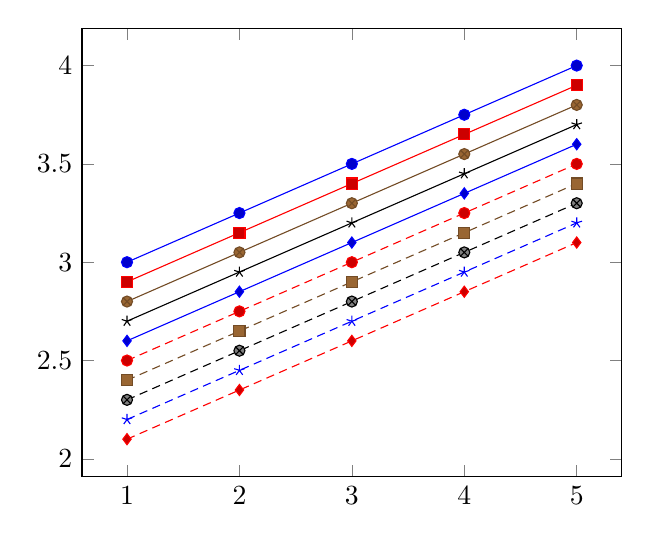
\begin{tikzpicture}
    \begin{axis}
      \foreach \y in {0,0.1,...,1} % Wiederholt \addplot mit jeweils anderem \y
        \addplot coordinates {
            ( 1, 3.0 -\y)
            ( 2, 3.25-\y)
            ( 3, 3.5 -\y)
            ( 4, 3.75-\y)
            ( 5, 4.0 -\y)
          };
    \end{axis}
  \end{tikzpicture}
  \caption{A beautiful plot.}%
  \label{fig:the-plot}
\end{figure}

\section{Conclusion}

Am Ende der Arbeit werden noch einmal die erreichten Ergebnisse
zusammengefasst und diskutiert.
